\section{L'arbre genealògic de FamilySearch}

    \paragraph{}
    El model de dades que conforma l'arbre genealògic de FamilySearch, consta de molts recursos i enumeracions diferents. No citem en la memòria el nombre total de recursos diferents, ja que alguns dels objectes documentats de forma oficial es troben en desús, mentre que alguns objectes nous, encara no han rebut la documentació pertinent.

    El conjunt d'objectes o recursos connectats, conformen el que ha estat enomenat l'arbre familiar de FamilySearch (Family Tree). Aquest arbre, pot ser subdividit en cinc grans blocs:

    \begin{itemize}
        \item \textbf{El bloc de persones:} Aquest bloc representa al conjunt de recursos que emmagatzemen la informació personal de les diferents persones representades a l'arbre familiar.
        \item \textbf{El bloc de les relacions familiars:} Aquest bloc està format per aquells recursos que contenen informació sobre les diferents relacions familiars entre les persones emmagatzemades en el sistema.
        \item \textbf{El bloc de col·leccions:} Aquest bloc recull els recursos que guarden la informació relativa a les fonts de dades i documents digitalitzats, que certifiquen la veracitat de les dades.
        \item \textbf{El bloc de discussions:} El bloc de discussions conté aquells recursos que contenen la informació relativa a les converses o discussions creades, per part dels usuaris, al voltant de les persones de l'arbre familiar.
        \item \textbf{El bloc de memòries:} Aquest últim bloc està format per aquells recursos que emmagatzemen la informació relativa a les memòries descrites en la secció tres d'aquesta memòria.
    \end{itemize}

    La imatge~\ref{fig:familyTree} mostra aquests cinc grans blocs que conformen l'arbre familiar de FamilySearch i com es troben relacionats entre ells.

    \begin{figure}[h]
        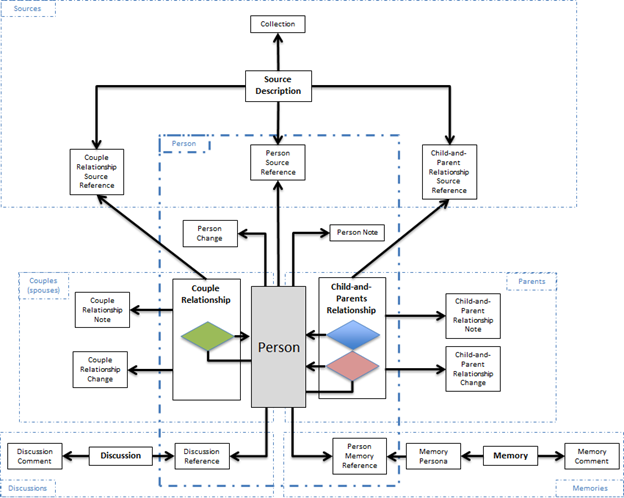
\includegraphics{05/02_overallModel}
        \centering
        \caption{Estructura de l'arbre familiar de FamilySearch}\label{fig:familyTree}
    \end{figure}

    Els blocs principals de l'arbre familiar són, sense cap mena de dubte, els que contenen la informació relativa a les persones i a les relacions familiars que les lliguen.

    L’objectiu de la resta de blocs que conformen l'arbre familiar és el de proporcionar suport i informació extra més detallada sobre les persones, relacions familiars, veracitat de les dades i investigacions realitzades sobre aquestes persones i línies genealògiques.

    En els següents apartats de la memòria s'estudiarà el conjunt de recursos principals que conformen cada bloc de l'arbre familiar i quines són les diferents peces d'informació accessibles a través de cada un d'aquests recursos.

    No es representarà en aquest projecte el conjunt total d'operacions diferents que pot ser realitzat sobre els diferents recursos, ja que les possibilitats de configuració d'aquestes són molt elevades i no té gaire sentit duplicar tota la documentació oficial respecte aquest punt.

    Tanmateix, sí que volem mencionar que gairebé tots els recursos que formen part del model de dades de FamilySearch, poden ser sotmesos als següents grups d'operacions:

    \begin{itemize}
        \item \textbf{Lectura:} Tots els recursos són, evidentment, llegibles. Cada un dels recursos conté diferents opcions de lectura i generalment, també solen ser personalitzables mitjançant la inclusió de diferents paràmetres.
        \item \textbf{Actualització:} Sempre que es disposi dels permisos adequats sobre les dades, els usuaris també poden realitzar operacions d'actualització per corregir errors, modificar la informació existent o bé afegir nova informació.
        \item \textbf{Esborrat:} Si es disposa dels permisos suficients, els usuaris poden esborrar informació incorrecta o duplicada dels diferents recursos, o el recurs sencer, mitjançant les operacions d'esborrat.
        \item \textbf{Creació:} En cas de voler afegir noves peces d'informació a les bases de dades de FamilySearch, siguin noves persones o informació específica relacionada a alguna persona que ja es troba en el sistema, això és realitzable a través de les operacions de creació de cada recurs.
    \end{itemize}

    Dit això, passem doncs a analitzar els principals recursos de cada bloc de l'arbre familiar i les peces d'informació més destacables que els conformen.
